\documentclass[a4paper]{article}

\usepackage[english]{babel}
\usepackage[utf8]{inputenc}
\usepackage{graphicx}
\usepackage[colorinlistoftodos]{todonotes}
\usepackage{xeCJK}
\usepackage{setspace}
\usepackage{amsmath}
\usepackage{upgreek}
\usepackage{amsfonts}
% \usepackage{txfonts}
\usepackage{dsfont}
\usepackage{multirow}
\usepackage{array}
\usepackage{setspace}
\usepackage{booktabs}
\usepackage{epsfig}
\usepackage{subfigure}
\usepackage{pythonhighlight}
\usepackage{float}
\usepackage{latexsym}
%\setCJKmainfont{SimSun}
\usepackage{geometry}
\usepackage{indentfirst}
\renewcommand{\baselinestretch}{1.2}
\geometry{a4paper,left=2.54cm,right=2.54cm,top=2.54cm,bottom=2.54cm}

\title{An Introduction to Tree Models}
\author{张春光\\WISER Club 2018, XMU}
\begin{document}
\setlength{\parindent}{2em}
\maketitle{}
\tableofcontents
% ================================================================================================
% ================================================================================================
% ================================================================================================
\section{Decision Tree}
% ================================================================================================
% ================================================================================================
	\subsection{基本概念}
	决策树模型可以分为决策树生成和决策树剪枝两个过程,决策树生成就是结点递归分裂产生叶结点的过程,
	决策树剪枝就是将某些叶结点移除的过程,所以决策树学习过程主要关注三点:
		\begin{itemize}
			\item 	结点如何分裂
			\item 	生成叶结点条件
			\item 	如何剪枝
		\end{itemize}
% ================================================================================================
% ================================================================================================
	\subsection{决策树分裂}
	结点分裂的目的是为了提升结点的纯度,使得分裂后子结点中所属的样本尽可能属于同一类别,减少数据集的不确定性。 
	目前不确定性衡量的方法有基于信息增益的信息论和统计检验方法。 基于信息论的方法主要有信息增益、信息增益率、
	基尼指数以及TwoValuing等,而基于统计检验的方法主要为卡方检验方法。
% ================================================================================================
		\subsubsection{离散属性}
		假定决策树中一结点$\mathbb{N}$中包含$k$个样本$\{(\textbf{x}_i,y_i)\,|\,i=1,2,\dots,n;\,y_i=1,2,\dots,k\}$,
		样本包含$k$类,每一类样本对应的比例为$p_k$,该结点可分裂的属性集合为$\mathcal{A}=\{\textbf{a}_i\,|\,i=1,2,\dots,m\}$,
		令$\mathbb{N}^{v}$为结点中属性$\textbf{a}$上取值为$a^v$的样本集合,定义$|\mathbb{N}|$为结点包含的样本容量。
			    \begin{itemize}
					\item[(1)]	信息增益\par
						定义结点的纯度指标信息熵(information entropy)为:
						$$\text{Ent}(\mathbb{N}) = -\sum_{i=1}^{k}p_i\log_2p_i$$
						结点的信息熵Ent$(\mathbb{N})$值越高,则结点纯度越高,则结点$\mathbb{N}$根据属性$\textbf{a}$进行分裂的
						信息增益为:
						$$\text{EntGain}(\mathbb{N},\,\textbf{a}) = \text{Ent}(\mathbb{N}) - \sum_{i=1}^{v}\frac{|\mathbb{N}^{i}|}{|\mathbb{N}|}\text{Ent}(\mathbb{N}^{i})$$
						则最优属性分裂为:
						$$\textbf{a}_{*} = \arg \max_{\textbf{a}}\text{EntGain}(\mathbb{N}, \textbf{a})$$
						即信息增益越大,样本纯度越高,分裂效果越好,考虑以下不等式:
						\begin{align*}
								-p_i\log_2p_i-p_j\log_2p_j+(p_i+p_j)\log_2(p_i+p_j) &= -p_i\log_2\frac{p_i}{p_i+p_j}-p_j\log_2\frac{p_j}{p_i+p_j}\\
																	&\geq 0+0 = 0\\
												-p_i\log_2p_i-p_j\log_2p_j 	&\geq -(p_i+p_j)\log_2(p_i+p_j)
						\end{align*}
						因此若一个属性$\textbf{a}$的取值数目越多,则该属性的信息增益会越高,在结点进行分裂时决策树会偏好取值较多的属性进行分裂,
						不过在样本量较大时可以不考虑该有偏性。
					\item[(2)] 	信息增益率\par
						由于信息增益在结点分裂时偏好取值数目多的属性进行划分,因此需要对属性的取值数目加一个惩罚项进行平衡,定义属性$\textbf{a}$的属性分离信息
						为:
						$$\text{SplitInfo}(\mathbb{N},\,\textbf{a}) = 
						       - \sum_{i=1}^{v}\frac{|\mathbb{N}^{i}|}{|\mathbb{N}|}\log_2\frac{|\mathbb{N}^{i}|}{|\mathbb{N}|}$$
						则结点$\mathbb{N}$根据属性$\textbf{a}$进行分裂的信息增益率:
						$$\text{EntGainRatio}(\mathbb{N},\,\textbf{a}) 
							= 	\frac{\text{EntGain}(\mathbb{N},\,\textbf{a})}{\text{SplitInfo}(\mathbb{N},\,\textbf{a})}
							= 	\frac{\text{Ent}(\mathbb{N}) - \sum_{i=1}^{v}\frac{|\mathbb{N}^{i}|}{|\mathbb{N}|}\text{Ent}(\mathbb{N}^{i})}{
							   -\sum_{i=1}^{v}\frac{|\mathbb{N}^{i}|}{|\mathbb{N}|}\log_2\frac{|\mathbb{N}^{i}|}{|\mathbb{N}|}}$$
						$\text{SplitInfo}(\mathbb{N},\,\textbf{a})$称为属性$\textbf{a}$的分离信息,在0和1两处接近于0且随着属性取值个数减少而减少,因此仅考虑属性的信息增益率进行分裂,则结点在分裂时会偏好取值较不平衡或取值个数较少的属性,因此一般使用信息增益率来筛选属性集合再用信息增益选取最优属性即
						最优属性分裂为:
						$$\textbf{a}_* = argmax_{\textbf{a}\in\{\textbf{a}_i|\,\text{EntGainRatio}(\mathbb{N},\,\textbf{a}_i)\geq 
										\text{mean}(\text{EntGainRatio}(\mathbb{N},\,\textbf{a}_i))\}}EntGain(\mathbb{N},\,\textbf{a})$$
						即先筛选出属性信息增益率高于平均信息增益率的属性集合,再计算信息增益选取最优属性。
					\item[(3)] 	基尼指数\par
						基尼指数一般用于二叉树模型中,表示结点分裂前后的基尼值的提升,基尼值直观理解为从结点中随机抽取两个样本不属于同一类的概率,因此基尼指数和信息熵不同,基尼指数越小表示结点纯度越高,即
						\begin{align*}
							   \text{Gini}(\mathbb{N}) &= 1 - \sum_{i=1}^{k}p_i^2\\
							   \text{GiniIndex}(\mathbb{N},\, \textbf{a}) &= \sum_{j=1}^{v}\frac{|\mathbb{N}^{j}|}{|\mathbb{N}|}\text{Ent}(\mathbb{N}^{j})		      
						\end{align*}
						$GiniIndex$从函数形式上也会偏好多值属性,但由于$GiniIndex$常用于二叉树,所以基本不考虑其属性有偏影响。
					\item[(4)] 	TwoingValue等\\
						$$\text{TwoingValue} = \frac{|\mathbb{N}_L|*|\mathbb{N}_R|}{|\mathbb{N}|^2}\left(\sum_{i=1}^{m}\left|\frac{L_i}{|\mathbb{N}_L|}-\frac{R_i}{|\mathbb{N}_R|}\right|\right)^2$$
						其中$L_i,\,R_i$表示属性$\textbf{a}_i$在左右结点$\mathbb{N}_L,\,\mathbb{N}_R$中的样本个数。
					\item[(5)] 	卡方检验:因基于信息论的属性选择有偏,QUEST及CHAID决策树算法基于卡方检验选择最优属性
						结点属性分裂的检验统计量为:
						$$G^2(\mathbb{N},\,\textbf{a}) = 2\ln2*|\mathbb{N}|\text{EntGain}(\mathbb{N},\,\textbf{a})\sim \chi_{U(\textbf{a})-1,|\mathbb{N}|-1}^2$$
						选取p--value值最低的属性作为最优分裂属性。
			    \end{itemize}
% ================================================================================================
		\subsubsection{连续属性}
			决策树从本质上来讲属于分类方法,因此对于连续属性特征的分裂需要先根绝属性的取值计算不同数值分裂的增益指标选取最优划分点,再与其他属性比较,具体计算如下:
			\begin{itemize}
				\item 	假定连续属性\textbf{a}有$v$个不同的取值$\{a^1,a^2,\dots,a^v\}$,先属性特征进行排序得到$\{a^{(1)},a^{(2)},\dots,a^{(v)}\}$;
				\item 	对于排序后的数列得到属性$\textbf{a}$的中值数列$T_a = \{\frac{a^{(1)}+a^{(2)}}{2},\frac{a^{(2)}+a^{(3)}}{2},\dots,\frac{a^{(v-1)}+a^{(v)}}{2}\}$,计算每个中值进行分裂的信息增益$EntGain(\mathbb{N},\,\textbf{a}, T_a)$:
					\begin{align*}
						\text{EntGain}(\mathbb{N},\,\textbf{a},\,t^*) 
								& = \max_{t\in T_a} \text{EntGain}(\mathbb{N},\,\textbf{a},\,t)\\
                    			& = \max_{t\in T_a} \left(\text{Ent}\left(\mathbb{N}\right) - 
                    				\sum_{\lambda \in \{L,R\}}\frac{|\mathbb{N}_\lambda^t|}{|\mathbb{N}|}\text{Ent}\left(\mathbb{N}_\lambda^t\right)\right)
					\end{align*}
				\item 	由于信息增益偏好多值属性,因此要对连续属性的信息增益进行修正,选择修正信息增益最大的分裂点作为该属性的划分点对数据划分:
					$$\text{EntGainRevise}(\mathbb{N},\,\textbf{a},\,t^*)  = \text{EntGain}(\mathbb{N},\,\textbf{a},\,t^*) - \frac{\log_2(v-1)}{|\mathbb{N}|}$$
			\end{itemize}
% ================================================================================================
		\subsubsection{缺失值}
			决策树对于缺失值的处理主要关注两点:
			\begin{itemize}
	        	\item 	\textbf{有缺失值的属性如何计算分裂指标}\\
	            	基于每个属性的无缺失样本$\bar{N}$计算信息增益或基尼系数,而后乘以无缺失比例:
	            	$$\text{EntGain}(\mathbb{N},\,\textbf{a}) = \rho \times \text{EntGain}(\bar{\mathbb{N}},\,\textbf{a}),\quad \rho = \frac{|\bar{\mathbb{N}}|}{|\mathbb{N}|}$$
	          	\item	\textbf{有缺失值的样本如何划分}\\
	            	在基于无缺失的样本属性选择之后,将每个缺失样本按照无缺失样本的后验概率的权重划分入各个子节点中。	
	        \end{itemize}
% ================================================================================================
	    \subsubsection{多变量组合划分}
	    	多变量决策树对于非叶结点划分时是对属性的线性组合进行测试,试图在每次属性划分时建立一个线性分类器,多变量决策树中较为常用的是CART Linear Combination算法,OC1算法(Oblique Classifier 1),其大致思想如下:
				\begin{itemize}
					\item 	CART Linear Combination\par
						\begin{itemize}
							\item[(1)] 先基于单变量选择最优属性$\textbf{x}_{j.}$,建立多变量组合分割平面H: $\sum_{i=1}^{m}a_ix_i+a_{m+1}=0$
							\item[(2)] 每次基于当前结点数据优化一个$\sum_{i=1}^{m}a_ix_i-\delta\left(x_i+\gamma\right)+a_{m+1}\leq0$,寻求最优$a_i,\,a_{m+1}$使得当前结点内的样本分类正确并更新;
							\item[(3)] Randomization; 因为在步骤(2)中每次更新$a_i$都是局部更新,因此在得到变量组合分割的超平面之后会进行扰动优化,生成
							随机向量$(r_1,r_2,\dots, r_{m+1})$加入超平面使得$H_1 = \sum_{i=1}^{m}\left(a_i+\alpha r_i\right)x_i+\left(a_{m+1}+r_{m+1}\right)$再次优化;
						\end{itemize}
					\item 	Recursive Least Square procedure
						\begin{align*}
						  	W_k &= W_{k-1}-K_k\left(X_k^TW_{k-1}-y_k\right)\\
						  	K_k &= P_kK_k\\
						  	P_k &= P_{k-1} - P_{k-1}X_k\left[1+X_k^TP_{k-1}X_k\right]^{-1}X_k^TP_{k-1}
						\end{align*}
					\item 	Feature Selection\par
						特征选取和回归中的stepwise类似采取SBE(Sequential Backward Elimination) 和SFE(Sequential Forward Selection)等, 以SBE为例,对具有
						n个属性的组合寻求最优参数,接下来依次删除其中一个属性,选择精度提高最多的一个属性进行剔除,以此类推,再用独立训练集验证;
				\end{itemize}
% ================================================================================================
% ================================================================================================
	\subsection{叶结点生成}
	决策树模型的最终目的是产生叶结点并进行预测,而在学习过程中产生叶结点的方式可分为以下几种形式:
	\begin{itemize}
	  	\item 	当前结点所含样本全部属于同一类别;
	  	\item 	当前结点属性值为空,没有其他属性进行划分,归类为结点中最多的所属类别;
	  	\item 	当前结点包含样本为空,样本分布参照父结点的样本分布;
	  	\item 	预剪枝。
	\end{itemize}
% ================================================================================================
% ================================================================================================
	\subsection{决策树剪枝}
	机器学习分类方法目的主要是为了提取某一类型样本的一般性特征,提高模型泛化识别能力,而非单一样例的个别特征,因此当决策树模型过深时,所产生的树模型往往会学习到个别特征,因此树模型一般需要进行剪枝处理来防止过拟合现象。
	\begin{itemize}
		\item 	预剪枝(阈值)\par
				预剪枝即在模型划分前对结点进行估计计算衡量指标,若不能提升则停止进行划分并标记为叶结点,
				预剪枝的优点在于模型训练的成本降低,但决策树训练时很多分支未展开导致存在欠拟合现象。预剪枝一般有以下几种形式:
				\begin{itemize}
					\item 	设定决策树最大深度;
					\item 	节点中的样本个数小于阈值;
					\item 	结点分裂的信息增益小于阈值。
				\end{itemize}
		\item 	后剪枝(损失函数)\par
				后剪枝即在模型训练生成完整一决策树时从下而上,对非叶结点进行替换为叶结点计算模型的泛化能力,若有提升则将将该结点替换为叶结点进行。
				从原理上来看,预剪枝寻求局部优化,而后剪枝以成本开销为代价寻求全局优化。预剪枝一般在模型构建中使用阈值来处理,而后剪枝一般使用树损失函数来进行剪枝。	
	\end{itemize}
% ================================================================================================
% ================================================================================================
	\subsection{决策树算法}
	决策树算法主要分为二叉树与多叉树模型,前者代表有CART和QUEST算法,后者有FACT、C4.5、CHAID、FRIM算法等。\\
	\noindent\rule[0.1\baselineskip]{\textwidth}{0.75pt}\\
	\textbf{Decision Tree Pseudo Code}\\
	\noindent\rule[0.1\baselineskip]{\textwidth}{0.5pt}\\
	\textbf{Input:}	Dataset $\textbf{D} = \{(\textbf{x}_i,\,y_i)\,|\,i = 1, 2,\dots, n;\, y_i = 1, 2, ..., k\}$;\\
	\hspace*{32pt}	Attributes $\textbf{A} = \{\textbf{a}_1,\textbf{a}_2,\dots, \textbf{a}_m\}$, Threshold $\epsilon$. \\
	\textbf{Procedure:}	TreeGenerate($\textbf{D},\,\textbf{A}$)\\
			\hspace*{32pt}	Generate a note $\mathbb{N}$\\
			\hspace*{32pt}	\textbf{if} all instance in $\mathbb{N}$ belong to a class j:\\
			\hspace*{48pt}	Label node $\mathbb{N}$ as Leaf Node of class j\\
			\hspace*{32pt}	\textbf{elif} $A = \emptyset$ or values of $\textbf{x}_{i}'s$ in $\mathbb{N}$ are same:\\
			\hspace*{48pt}	Label node $\mathbb{N}$ as Leaf Node of the class which has the most instance in $\mathbb{N}$ \\
			\hspace*{32pt}	Select a optimal partitioning attributes $\textbf{a}_*$\\
			\hspace*{32pt}	\textbf{if} $\text{Gain}(\mathbb{N},\,\textbf{a}_*) < \epsilon$:\\
			\hspace*{48pt}	\textbf{pass}\\
			\hspace*{32pt}	\textbf{for} value $a_*^{v}$ in $\textbf{a}_*$:\\
			\hspace*{48pt}	Generate branch for $\mathbb{N}$, denote $\mathbb{N}_v$ as subsample of $\mathbb{N}$ which have value $a_*^{v}$\\
			\hspace*{48pt}	\textbf{if} $\mathbb{N}_v$ is empty: \\
			\hspace*{64pt}	Label node $\mathbb{N}$ as Leaf Node of class j\\
			\hspace*{48pt}	\textbf{else}:\\
			\hspace*{64pt}	Denote TreeGenerate($\mathbb{N}_v,\, \textbf{A}\slash\textbf{a}_*$) as child node;\\
	\textbf{Output:} An Decision Tree $\mathbb{T}$\\
	\noindent\rule[0.1\baselineskip]{\textwidth}{0.75pt}
% ================================================================================================
		\subsubsection{ID3}
		最早的决策树类型,采用信息增益指标进行评估和特征选择,也较为粗糙。
		  	\begin{itemize}
		    	\item 	最优属性分割指标:信息增益;
		    	\item 	连续属性处理:无法处理;
		    	\item 	缺失值处理:无法处理;
		    	\item 	剪枝:未进行后剪枝处理;
		    	\item 	适用:数据存于内存中,小规模数据集。
		  	\end{itemize}
		FIRM算法则是在ID3算法上每个连续性属性划分为10个属性在进行树的生成, 也不进行剪枝。	
% ================================================================================================	
		\subsubsection{C4.5}
		C4.5决策树算法继承ID3决策树并进行改进:
		\begin{itemize}
		    \item 	最优属性分割指标:\textbf{结合信息增益和信息增益率进行属性划分选择,避免偏好取值多的属性;};
		    \item 	属性处理:二分法对连续属性离散化处理,对离散属性则采用多分法; 
		    \item 	缺失值处理:根据后验概率分配到子结点;
		    \item 	剪枝:采用悲观剪枝法(Pessimistic Error Pruning)
		    	悲观剪枝法主要是在决策树学习过程中通过训练集在结点分裂前后考察决策树的修正误差作为指标,决定是否生成该节点,其中修正误差为
		    	决策树的误判样本数目加上叶结点数目作为惩罚项,可近似将决策树修正误差当作二项分布来考察:
		    	\begin{enumerate}
		    		\item 	定义$\|\mathbb{T}\|$为决策树$\mathbb{T}$的叶结点数目,$\epsilon(\mathbb{T})$为决策树的误判样本数目;
					\item 	对任意内部结点$\mathbb{N}$, 包含样本个数为$|\mathbb{N}|$, 假定该结点根据最优属性划分生成子树为$\mathbb{T}_{\mathbb{N}}$;
					\item 	计算将结点$\mathbb{N}$作为叶结点的模型修正错误率:
							$$\epsilon^{'}(\mathbb{N}) = \epsilon(\mathbb{N}) +\frac{\|\mathbb{N}\|}{2}=\epsilon(\mathbb{N}) +\frac{1}{2}$$
					\item 	计算将结点$\mathbb{N}$作为内部结点即子树$\epsilon(\mathbb{T})$的错误率以及标准差:
							\begin{align*}
								\epsilon^{'}(\mathbb{T}_{\mathbb{N}}) 	&= \epsilon(\mathbb{T}_{\mathbb{N}}) +\frac{\|\mathbb{T}_{\mathbb{N}}\|}{2}\\
							SE[\epsilon^{'}(\mathbb{T}_{\mathbb{N}})]	&= \sqrt{\frac{\epsilon^{'}(\mathbb{T}_{\mathbb{N}})
											\left(|\mathbb{N}|-\epsilon^{'}\left(\mathbb{T}_{\mathbb{N}}\right)\right)}{|\mathbb{N}|}}
							\end{align*}
					\item 	对比结点分裂前后的误差:
							$$G(\mathbb{N}) = \epsilon^{'}(\mathbb{T}_{\mathbb{N}})+SE[\epsilon^{'}(\mathbb{T}_{\mathbb{N}})]-\epsilon^{'}(\mathbb{N})$$
							若$G(\mathbb{N})\geq0$则进行剪枝,将内部结点$\mathbb{N}$作为叶结点,反之则不剪枝。
				\end{enumerate} 
		    \item 适用:在构造树时需要对数据的属性进行多次扫描和排序,占内存、低效。
		  \end{itemize}
% ================================================================================================
		\subsubsection{CART}
		CART决策树为分类与回归树,假定决策树是二叉树,内部结点特征为是和否,递归二分每个特征,在进行回归时使用叶结点的样本的均值输出预测值;
		\begin{itemize}
			\item 	最优属性分割指标:使用GINI系数进行属性划分;
			\item 	属性处理:对于连续属性采用多次二分法,离散属性划分时每次选择其中一种分割数据,对属性特征重复性使用;
			\item 	对于多分类目标,会将目标类别合并成两个超类别;
			\item 	对于树的构建,CART算法会生成尽量大的数目,而后用验证数据集根据损失函数对已生成的树进行剪枝,选择最优子树;
			\item 	剪枝:采用独立的验证集剪枝处理,否则剪枝结果为深度最大的子树;
				\begin{enumerate}
					\item 	定义决策树$\mathbb{T}$的损失函数$\ell(\mathbb{T})$:
						\begin{align*}
							\ell_{\alpha}(\mathbb{T}) 
								& = \ell(\mathbb{T}) + \alpha\|\mathbb{T}\| 
								  = \sum\nolimits_{t=1}^{\|\mathbb{T}\|}|\mathbb{N}_t|H_{\mathbb{N}_t} + \alpha\|\mathbb{T}\|\\
							H_{\mathbb{N}}
								& = -\sum_k\frac{|\mathbb{N}^k|}{|\mathbb{N}|}\log\frac{|\mathbb{N}^k|}{|\mathbb{N}|}
						\end{align*}
						$\alpha$为树模型复杂度的惩罚系数, $\|\mathbb{T}\|$为决策树叶结点数目, $|\mathbb{N}|$为叶结点$\mathbb{N}$上的样本数,
						$|\mathbb{N}^k|$为叶结点$\mathbb{N}$上为类k的样本数,$H_{\mathbb{N}}$为叶结点$\mathbb{N}$上的经验熵
					\item 	对整棵树分别计算以任意内部结点$\mathbb{N}$为单结点的树$\mathbb{N}$和根节点的树$\mathbb{T}_{\mathbb{N}}$的损失
						$$\ell_\alpha(\mathbb{N}) = \ell(\mathbb{N})+\alpha\|{\mathbb{N}}\| = \ell(\mathbb{N})+\alpha,
						\quad \ell_\alpha(\mathbb{T}_{\mathbb{N}}) = \ell(\mathbb{T}_{\mathbb{N}})+\alpha\|\mathbb{T}_{\mathbb{N}}\|$$
					\item 	当且仅当$\ell_\alpha(\mathbb{N})\leq \ell_\alpha(\mathbb{T}_{\mathbb{N}})$时,决策树会进行剪枝剪除$\mathbb{T}_{\mathbb{N}}$,
						将$\mathbb{N}$作为叶结点;
					\item 	令$G(\mathbb{N}) = \frac{\ell_\alpha(\mathbb{N})-\ell_\alpha(\mathbb{T}_{\mathbb{N}})}{\|\mathbb{T}_{\mathbb{N}}\|-1}$,
						计算所有内部结点$\mathbb{N}$的$G(\mathbb{N})$值,依次增加$\alpha$,自下而上递归在决策树$\mathbb{N}_i$中剪除$G(\mathbb{N}_i)$最小的$\mathbb{T}_{\mathbb{N}^i}$得到$\mathbb{N}_{i+1}$子树;
					\item 利用独立测试集计算独立子树集合$\{\mathbb{N}_i\}$的损失函数$\ell(\mathbb{N}_i)$,取最优子树$\mathbb{N}_i^{*}$。
				\end{enumerate}
			\item 	Scikit\-learn 模块中使用的决策树算法为CART算法:\par
					$\textbf{DecisionTreeClassifier}(\text{criterion}=gini,\, \text{splitter}=best,\, \text{max\_depth}=None, \\
					\hspace*{12pt}\text{min\_samples\_split}=2,\, \text{min\_samples\_leaf}=1,\, \text{min\_weight\_fraction\_leaf}=0,\\
					\hspace*{12pt}\text{max\_features}=None,\, \text{random\_state}=None,\, \text{max\_leaf\_nodes}=None, \\
					\hspace*{12pt}\text{min\_impurity\_decrease}=0.0,\, \text{min\_impurity\_split}=None,\\
					\hspace*{12pt}\text{class\_weight}=None,\, \text{presort}=False)$\\
					多数指标都是针对剪枝进行改进。
			\item 	\textbf{CART回归树}\par
				主要先将决策树的输出空间划分为M个空间$R_1,R_2,\dots,R_m$, 每个空间对应输出值$c_1,c_2,\dots,c_m$,而在
				对属性$\textbf{a}$选择和切分点$a^v$时不是选择信息增益或基尼指数,而是最小化:
				$$\min_{\textbf{a},\,a^v}\left[\min_{c_1}\sum\nolimits_{x_i\in \{x|x^a\leq a^v\}}\left(y_i-c_1\right)^2+
											   \min_{c_2}\sum\nolimits_{x_i\in \{x|x^a> a^v\}}\left(y_i-c_2\right)^2\right]$$
				其中$c_i$在平方误差损失函数下一般取值为$R_i$区间内样本的均值。	
		\end{itemize}
% ================================================================================================
% ================================================================================================
% ================================================================================================
\section{Bagging}
% ============================================================================================================================================
	\subsection{RandomTreesEmbedding}
		Bagging结合Bootstrap,使得模型有部分验证集对组合学习器进行包外估计,可以起到降低方差的效果,不易受干扰。
		\begin{align*}
			\text{Dataset D}	& \Rightarrow \text{Bootstrap m subsets}\{D_1, D_2,\dots, D_m\}\\
					  			& \Rightarrow \text{Train m learner}\,\{\mathbb{H}_i(\textbf{x},\, i=1,2,\dots, m)\}\\
					  			& \Rightarrow H(\textbf{x}) = \arg\max \sum\nolimits_{i=1}^{m}\mathbb{I}\left(\mathbb{H}_i(\textbf{x})=y\right)
		\end{align*}
% ============================================================================================================================================
	\subsection{RandomForest}
	随机森林在RandomTreesEmbedding上基础上进行改进,在构建每克决策树过程中引入\textbf{随机属性选择}.传统决策树在选择属性划分时候对当前结点的属性集合(d)中
	选择最优属性,而在随机森林中,先对当前结点的属性集合中随机选择k(多数情况下为$\log_2d$)个属性子集,然后再从属性子集中选择最优属性。
% ============================================================================================================================================
	\subsection{StackingStrategy}
		Average, WeightedAverage, Majority Vote, MetaLearnerStacking,\dots
% ================================================================================================
% ================================================================================================
% ================================================================================================
\section{Boosting}
	\subsection{基本概念}
	\begin{itemize}
		\item Boosting 基本流程:
		Boosting是一种基于改变原始数据集分布的迭代串行组合算法,主要流程:
			\begin{itemize}
				\item[(1)]	从初始训练集用初始权重训练出一个基学习器$\mathbb{H}_1$,得到训练集输出值$h(\textbf{x})$;
				\item[(2)]	根据基学习器的学习误差率$\epsilon_1$调整更新训练样本权值$\upomega$,使得误差率高的训练样本权值$\omega$增加,并确定该学习器的权重$\alpha_1$;
				\item[(3)]	基于新的样本权值训练基学习器$\mathbb{H}_2$;
				\item[(4)]	迭代步骤2和3,直到基学习器数目到达预设数目t,然后根据基学习器的权重$\upalpha$组合基学习器的训练结果输出;
				\begin{figure*}[h]
					\centering
					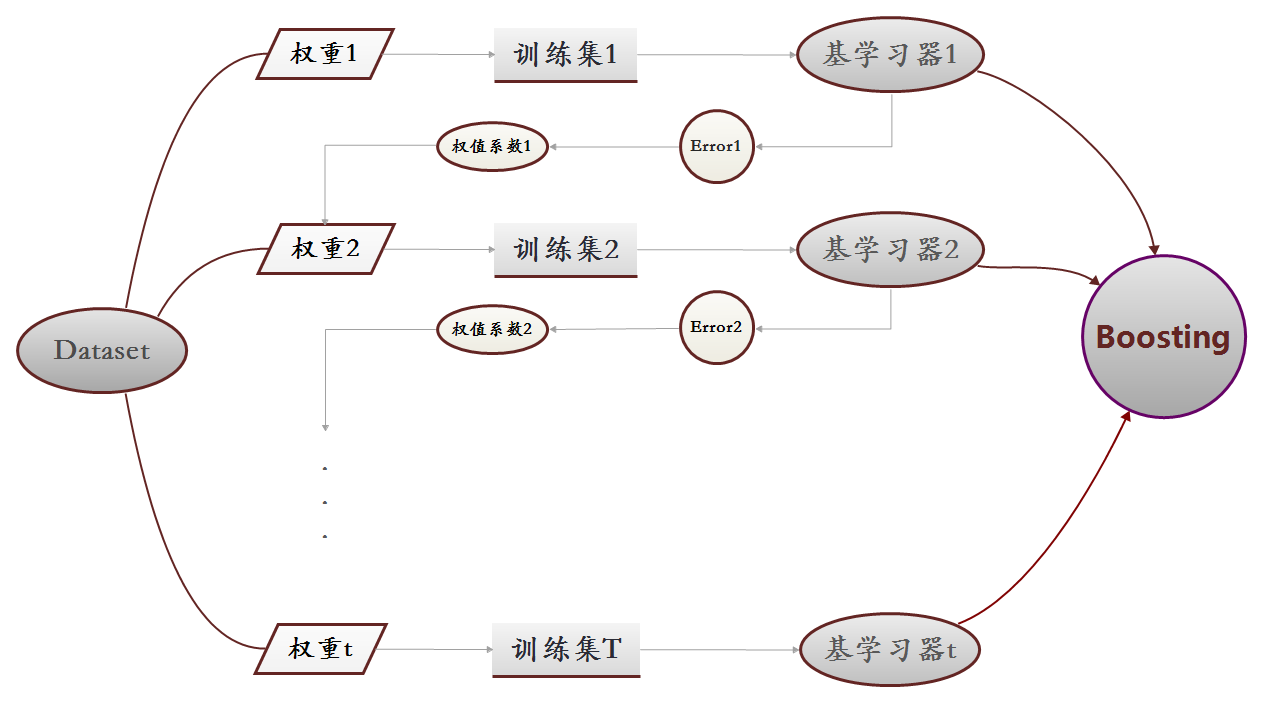
\includegraphics[width=0.75\textwidth]{Dataset.png}
					\caption{Boosting}
				\end{figure*}
			\end{itemize}
			所以不同的Boosting方法的区别在于以下几点:
			\begin{itemize}
				\item 学习误差率的计算方式即Loss function形式$\ell$;
				\item 如何根据误差率更新样本权重系数$\upomega$;
				\item 如何确定基学习器的权重系数$\upalpha$;
			\end{itemize}
			针对多数Boosting算法,基本都是采用加法模型组合弱分类器,用前向分布算法来更新训练数据的权重和概率分布进行模型学习。

		\item 前向分布算法
		前向分布算法是一个组合算法优化的一种求解方案,主要思路是通过从前向后每次学习一个基函数及其系数,逐步逼近优化目标函数来简化组合算法的优化复杂度。
			\begin{itemize}
				\item[(1)] 	考虑由t个基学习器组成的Boosting加法模型:$$\hat{\mathbf{y}}^t = \sum_{i=1}^{t}\beta_{i}h^i(\textbf{x})$$
				\item[(2)]	解决这一优化问题可采用前向分布算法从前往后每次只学习一个基函数及其系数,逐步逼近优化目标函数来简化复杂度,即
				$${Obj}^{(t)} = \sum_{i=1}^{n}\ell\left(y_i, \hat{y}_i^t\right)+\sum_{i=1}^{t}\Omega(\mathbb{H}_i) 
								   = \sum_{i=1}^{n}\ell\left(y_i, \hat{y}_{i}^{t-1}+h_i^t(\textbf{x})\right)+\Omega(\mathbb{H}_t))+\text{Const.}$$
				\item[(3)]	因此,最优化目标函数就转化为基于前一学习器的预测来最优化当前损失函数,即最小化
				$$\sum_{i=1}^{n}\ell\left(y_i, \hat{y}_{i}^{t-1}+h_i^t(\textbf{x})\right)+\Omega(\mathbb{H}_t)$$
				\item[(4)]	以平方损失函数为例,则模型转为拟合上一轮的残差:
				$$\sum_{i=1}^{n}\left(y_i-\hat{y}_{i}^{t-1}+h_i^t(\mathbf{x}_i))^2+\Omega(\mathbb{H}_t\right) 
						= \sum_{i=1}^{n}\left(-\epsilon_i^{t-1}+h_i^t(\mathbf{x})\right)^2 + \Omega(\mathbb{H}_t)$$
				\item[(5)] 	而损失函数$\ell$的形式及其泰勒展开项数的不同产生就衍生出不同的Boosting算法。
			\end{itemize}
	\end{itemize}
	\subsection{AdaBoost}
	AdaBoost即adaptive boosting,可视为损失函数为指数函数、学习算法为前向分步算法的二分类加法模型,
	顾名思义即通过调整训练样本的权值分布,为弱学习器定义不同的权值,将其线性组合成一个强学习器。
	\begin{align*}
		f(\textbf{x}) 
			& = \sum_{i=1}^{t}\alpha_th_t(\textbf{x})\\
   		\ell_{\exp}(y,f(\textbf{x})|\upomega)
   			& = E_{\textbf{x}\sim\upomega}[\exp(-\textbf{y} f(\textbf{x}))]
	\end{align*}
	之后经过发展衍生出用于解决多分类的AdaBoost.m系列算法以及用于回归问题的AdaBoost.r系列算法。
		\subsubsection{AdaBoost for Binary Classification}
		AdaBoost的主要特点在于:
		\begin{itemize}
				\item 权值更新:
					$\omega_{t+1} \sim \omega_t\exp(-\alpha_t\textbf{y} f(\textbf{x}))$\\
					即若分类正确权值同比于上一轮的$\exp(-\alpha)$,若分类错误权值增大为上一轮$\exp(\alpha)$;
				\item 基学习器权值与样本权值更新系数:
					$\alpha_t = \frac{1}{2}\ln \frac{1-\epsilon_t}{\epsilon_t}$\\
					单个基学习器分类误差率越低,权值越高。
		\end{itemize}
			\noindent\rule[0.1\baselineskip]{\textwidth}{0.75pt}\\
			\textbf{Algorithm: AdaBoost for Binary Classification}\\
			\noindent\rule[0.1\baselineskip]{\textwidth}{0.5pt}\\
			\textbf{Input:} Dataset $\textbf{D} = \{(\mathbf{x}_i,\,y_i)\,|\,i = 1, 2,\dots, n;\, y_i = -1, 1\}$\\
			\hspace*{32pt} WeakLearner $\mathbb{H}$, Loss function $\ell$, Iterations $T$\\
			\textbf{Procedure:} \\
					\hspace*{32pt}	$\upomega_1(\textbf{x}) = \frac{1}{n}$\\
					\hspace*{32pt}	\textbf{for} $t = 1, 2,\dots, T$:\\
							\hspace*{48pt}	$h_t(\textbf{x}) = \mathbb{H}(\textbf{D}, \upomega)$\\
							\hspace*{48pt}	$\epsilon_t = \ell(\textbf{y}, h_t(\textbf{x})) = P_{\textbf{x}\sim\upomega_t}(h_t(\textbf{x}) \neq \textbf{y})$\\
							\hspace*{48pt} 	\textbf{if} $\epsilon_t > 0.5$: \\
							\hspace*{64pt}	\textbf{break}\\
							\hspace*{48pt} 	$\alpha_t = \frac{1}{2}\ln\frac{1-\epsilon_t}{\epsilon_t}$\\
							\hspace*{48pt} 	$\upomega_{t+1} = \frac{\upomega_t(\textbf{x})}{Z_t}\exp\left(-\alpha_t\textbf{y}h_t(\textbf{x})\right),
													\, Z_t = E_{\textbf{x}\sim \upomega_t}(\textbf{x})\exp(-\alpha_t\textbf{y}h_t(\textbf{x}))$\\
			\textbf{Output:} $f(\textbf{x}) = \sum_{i=1}^{t}\alpha_th_t(\textbf{x})$\\
			\noindent\rule[0.25\baselineskip]{\textwidth}{0.75pt}
			\begin{itemize}
				\item 指数损失函数$\ell(\mathbf{y}, f(\textbf{x}))$最小化
					\begin{align*}
						\frac{\partial \ell_{\exp}(f(\textbf{x})|\upomega)}{\partial f(\textbf{x})}
							& = \frac{\partial E_{\textbf{x}\sim\upomega}[\exp(-\textbf{y} f(\textbf{x}))]}{\partial f(\textbf{x})}\\
							& = \frac{\partial \left(\exp(-f(\textbf{x}))P(\textbf{y}=1|\textbf{x})+
													\exp(f(\textbf{x}))P(\textbf{y}=-1|\textbf{x})\right)}{\partial f(\textbf{x})}\\
							& = -\exp(-f(\textbf{x}))P(\textbf{y}=1|\textbf{x})+\exp(f(\textbf{x}))P(\textbf{y}=-1|\textbf{x})=0\\
						f(\textbf{x}) 
							& = \frac{1}{2}\ln\frac{P\left(f(\textbf{x})=1|\textbf{x}\right)}{P\left(f(\textbf{x})=-1|\textbf{x}\right)}\\
						\text{sign}(f(\textbf{x})) 
							& = \text{sign}\left[\frac{1}{2}\ln\frac{P\left(f(\textbf{x})=1|\textbf{x}\right)}{P\left(f(\textbf{x})=-1|\textbf{x}\right)}\right] \\
							& = \left \{\begin{array}{ll}
											1,\, &P(f(\textbf{x})=1|\textbf{x}) > P(f(\textbf{x})=-1|\textbf{x})\\
										   -1,\, &P(f(\textbf{x})=1|\textbf{x}) < P(f(\textbf{x})=-1|\textbf{x})
										\end{array} \right.\\
							& = \arg \max_{y\in \{-1,1\}} P(f(\textbf{x})=\mathbf{y})
						\end{align*}
				也即指数损失函数最小化等同于二分类方法中最大化分类正确率。
				\item 误差率$\epsilon_t$更新权值系数$\alpha_t$
					\begin{align*}
						\ell_{\exp}(\alpha_t h_t(\textbf{x})|\upomega_t) 
							& = E_{\textbf{x}\sim\upomega_t}[\exp(-\alpha_t\textbf{y}h_t(\textbf{x})] \\
							& = E_{\textbf{x}\sim\upomega_t}[\exp(-\alpha_t)\mathbb{I}(\textbf{y}=h_t(\textbf{x}))+
						 		\exp(\alpha_t)\mathbb{I}(\textbf{y} \neq h_t(\textbf{x}))] \\
							& = \exp(-\alpha_t)(1-\epsilon_t) + \exp(\alpha_t)\epsilon_t\\
						\frac{\partial \ell_{\exp}(\alpha_th_t(\textbf{x}))}{\partial \alpha_t}
							& = -\exp(-\alpha_t)(1-\epsilon_t) + \exp(\alpha_t)\epsilon_t = 0 \\
						\alpha_t 
							& = \frac{1}{2}\ln\frac{1-\epsilon_t}{\epsilon_t}
					\end{align*}
				\item 前向分布算法推导$h_t(\textbf{x}),\,\upomega_t$
					\begin{align*}
						h_t(\textbf{x}) 
							& = \arg\min_h \ell_{\exp}\left(\textbf{y},f_{t-1}(\textbf{x})+\alpha_th_t(\textbf{x})|\upomega\right) \\
							& = \arg\min_h E_{\textbf{x}\sim\upomega}\left[\exp(-\alpha_t\textbf{y}f_{t-1}(\textbf{x}))\exp(-\textbf{y}\alpha_th_t(\textbf{x}))\right]\\
							& = \arg\min_h E_{\textbf{x}\sim\upomega}\left[\exp(-\alpha_t\textbf{y}f_{t-1}(\textbf{x}))\exp(-\textbf{y}\alpha_th_t(\textbf{x}))\right]\\
				   			& \equiv \arg\min_h E_{\textbf{x}\sim\upomega}\left[\exp\left(-\alpha_t\textbf{y}f_{t-1}(\textbf{x})\right)
				   									\left(1-\textbf{y}h_t(\textbf{x}) + \frac{\textbf{y}^2h_t^2(\textbf{x})}{2}\right)\right]\\
				   			& = \arg\min_h E_{\textbf{x}\sim\upomega}\left[\exp(-\alpha_t\textbf{y}f_{t-1}(\textbf{x}))\left(1-\textbf{y}h_t(\textbf{x})+\frac{1}{2}\right)\right] \\
				   			& = \arg\min_h E_{\textbf{x}\sim\upomega}\left[\frac{\exp(-\alpha_t\textbf{y}f_{t-1}(\textbf{x}))}
				   									{E_{\textbf{x}\sim\upomega}[\exp(-\textbf{y}f_{t-1}(\textbf{x}))]}\textbf{y}h_t(\textbf{x})\right] \\
				   			& = \arg\min_h E_{\textbf{x}\sim\upomega_t}[\textbf{y}h_t(\textbf{x})], \, \text{where}\, \upomega_t(\textbf{x})|\upomega = 
				   				\frac{\upomega\exp(-\alpha_t\textbf{y}f_{t-1}(\textbf{x}))}{E_{\textbf{x}\sim\upomega}[\exp(-\alpha_t\textbf{y}f_{t-1}(\textbf{x}))]} \\
						   	& = \arg\min_h E_{\textbf{x}\sim\upomega_t}[1-2\mathbb{I}(\textbf{y}\neq h_t(\textbf{x}))]\\ 
						   	& = \arg\max_h E_{\textbf{x}\sim\upomega_t}[\mathbb{I}(\textbf{y}= h_t(\textbf{x})]\\
		   				\upomega_{t+1} 	
		   					& = \frac{\upomega_t\exp(-\alpha_t\textbf{y}f_t(\textbf{x}))}{E_{\textbf{x}\sim\upomega_t}[\exp(-\alpha_t\textbf{y}f_{t}(\textbf{x}))]} \\
		   		   			& = \upomega_t\exp(-\alpha_t\textbf{y}h_{t}(\textbf{x})))\frac{E_{\textbf{x}\sim \upomega_t}
		   		   				[\exp(-\alpha_t\textbf{y}f_{t-1}(\textbf{x}))]}{E_{\textbf{x}\sim \upomega_t}[\exp(-\alpha_t\textbf{y}f_{t}(\textbf{x}))]}\\
		   		   			& = \upomega_{t-1}\frac{\exp(-\alpha_t\textbf{y}f_t(\textbf{x}))\exp(-\alpha_{t-1}\textbf{y}f_{t-1}(\textbf{x}))}{Z_tZ_{t-1}}=\cdots
					\end{align*}
			\end{itemize}
			\par AdaBoost作为弱分类器的组合器,基分类器越弱,效果提升越明显,不容易过拟合,且基于AdaBoost框架可以拓展回归和多分类问题。
			但由于AdaBoost的权值更新方式的原理,AdaBoost对异常数据比较敏感,因异常数据在不断迭代中往往会获得较高的权值,
			最终影响模型预测准确性。
		\subsubsection{AdaBoost.M for Multiple Classification}
			AdaBoost基本算法仅应用于二分类方法,因此在面对多分类问题需要在权重更新方式上进行改进。\\
			\noindent\rule[0.1\baselineskip]{\textwidth}{0.75pt}\\
			\textbf{AdaBoost.m1 for Multiclass Classification}\\
			\noindent\rule[0.1\baselineskip]{\textwidth}{0.5pt}\\
			\textbf{Input:} Dataset $\textbf{D} = \{(\mathbf{x}_i,\,y_i)\,|\,i = 1, 2,\dots, n;\, y_i = 1, 2, \dots, k\}$\\
			\hspace*{32pt} WeakLearner $\mathbb{H}$, Loss function $\ell$, Iterations $T$\\
			\textbf{Procedure:} \\
					\hspace*{32pt}	$\upomega_1(\textbf{x}) = \frac{1}{n}$\\
					\hspace*{32pt}	\textbf{for} $t = 1, 2,\dots, T$: \\
							\hspace*{48pt}	$h_t(\textbf{x}) = \mathbb{H}(\textbf{D}, \upomega)$\\
							\hspace*{48pt}	$\epsilon_t = \ell(\textbf{y}, h_t(\textbf{x})) = P_{\textbf{x}~\upomega_t}(h_t(\textbf{x}) \neq \textbf{y})$\\
							\hspace*{48pt}	\textbf{if} $\epsilon_t > 0.5$: \\
							\hspace*{64pt}	\textbf{break}\\
					        \hspace*{48pt}	$\alpha_t = \ln\frac{1-\epsilon_t}{\epsilon_t}$\\
					        \hspace*{48pt}	$\upomega_{t+1} = \frac{\upomega_t}{Z_t}\exp(-\alpha_t(1-[h_t(\textbf{x})\neq \textbf{y}]))$\\
					\textbf{Output:} $f(\textbf{x}) = \sum_{t=1}^{T}\alpha_t[h_t(\textbf{x})=\textbf{y}]$\\
			\noindent\rule[0.1\baselineskip]{\textwidth}{0.75pt}\\
			从算法中可以看出AdaBoost.m1仅在权值更新时对判断正确的样本调低权重为原有的$\exp(-\alpha_t)$,而对于判断错误的样本权值不进行更新,从而增加误分类的权值。
			与AdaBoost相比较而言:
				\begin{itemize}
					\item 样本权值放缩权值降低,二分类中以$\exp(2\alpha_t)$的扩张系数更新误判样本的权值,而AdaBoost.m1以$\exp(\alpha_t)$的系数增加;
					\item AdaBoost.m1仅考虑样本是否分类错误,但不考虑被误判为其他一类别,而二分类中由于只有两个类别不存在此缺陷;
					\item AdaBoost.m1也会受到异常值的影响,特别是多分类不平衡的数据难以产生好的效果。
				\end{itemize}
		\subsubsection{AdaBoost.M2 for Multiple Classification}
			AdaBoost.M2则是基于AdaBoost.M1的基础上进行改进,比较AdaBoost.M1只考虑是否分类正确而言,该更新权值考虑两方面:
			\begin{itemize}
				\item 先是根据判断样本是否分类正确,从而调整权值;
				\item 再是根据错误样本误判为其他类别,调整其他类别样本的权重;
			\end{itemize}
			\noindent\rule[0.1\baselineskip]{\textwidth}{0.75pt}\\
			\textbf{AdaBoost.m2 for Multiclass Classification}\\
			\noindent\rule[0.1\baselineskip]{\textwidth}{0.5pt}\\
			\textbf{Input:} Dataset $\textbf{D} = \{(\mathbf{x}_i,\,y_i)\,|\,i = 1, 2,\dots, n;\, y_i = 1, 2, \dots, k\}$\\
			\hspace*{32pt} WeakLearner $\mathbb{H}$, Loss function $\ell$, Iterations T\\
			\textbf{Procedure:} \\
					\hspace*{32pt}  $\Upomega^1 = \frac{1}{n}$\\
					\hspace*{32pt}	$\upomega_{i,y}^{1} = \frac{\Upomega^1}{k-1}$ for $i = 1,2,\dots,n\,\,\text{and}\,\, y\neq y_i$\\
					\hspace*{32pt}	\textbf{for} i = 1,2,\dots,T: \\
					\hspace*{48pt}	$\textbf{w}_i^t = \sum_{y\neq y_i}\omega_{i,y}^t$\\
					\hspace*{48pt}	$q_{i,y}^t = \frac{\upomega_{i,y}^{t}}{\textbf{w}_i^t}$ for $y\neq y_i$\\
					\hspace*{48pt}	$\Upomega_t = \frac{\textbf{w}_i^t}{\sum_{i=1}^{n}\textbf{w}_i^t}$\\
					\hspace*{48pt}	$h^t(\textbf{x}, \textbf{y}) = \mathbb{H}(\textbf{D}, \Upomega_t)$\\
					\hspace*{48pt}	$\epsilon_t = \frac{1}{2}\sum_{i=1}^{n}\Upomega^t_i(1-h^t_i(\textbf{x},y_i)+\sum_{i,y\neq y_i}q_{i,y}^th^t_i(\text{x},y))$\\
					\hspace*{48pt}	\textbf{if} $\epsilon_t > 0.5$:\\
					\hspace*{64pt}	\textbf{break}\\
					\hspace*{48pt}	$\alpha_t = \ln\frac{1-\epsilon_t}{\epsilon_t}$\\
					\hspace*{48pt}	$\upomega_{i,y}^{t+1} = \upomega_{i,y}^t\exp(-\frac{1}{2}\alpha_t(1+h_t(\textbf{x},y_i)-h_t(\textbf{x},y)))$ for $y\neq y_i$\\
			\textbf{Output:} $f(\textbf{x}) = \sum_{t=1}^{T}\alpha_th_t(\textbf{x},y)$\\
			\noindent\rule[0.1\baselineskip]{\textwidth}{0.75pt}\\
			算法中的符号含义:
			\begin{itemize}
				\item $\Upomega^t$: 表示第t个学习器输入的训练数据样本的权值,大小为$n\times 1$;
				\item $\upomega_{i,y}^{t}$: 表示第t个学习器输入的第i个样本里若被错判为其他类别的损失权重;
				\item $\textbf{w}_i^t$: 表示不属于$y_i$类别的样本权重之和,这里是为了Normalize权重;
				\item $q_{i,y}^t$: Normalized $\upomega_{i,y}^{t}$。
			\end{itemize}
			算法中学习器$\mathbb{H}(\textbf{D}, \Upomega_t)$输出一个$n\times k$浮点数矩阵而不是AdaBoost中的类别,
			而在计算误差率时要根据被错判的类别$h^t(\text{x}_i,y_i)$、易被错归类的类别$h^t(\text{x}_i,y)$及
			其损失权重$q_{i,y}^t$计算总损失双向更新权重。
		\subsubsection{AdaBoost.R1 for Regression}
			AdaBoost.R1则是基于AdaBoost算法应用于回归问题的改进。\\
			\noindent\rule[0.1\baselineskip]{\textwidth}{0.75pt}\\
			\textbf{AdaBoost.R for Regression}\\
			\noindent\rule[0.1\baselineskip]{\textwidth}{0.75pt}\\
			\textbf{Input:}	Dataset $\textbf{D} = \{(\textbf{x}_i,\,y_i)\,|\,i = 1, 2,\dots, n;\, y_i \in [0,\,1]\}$\\
			\hspace*{32pt}	WeakLearner $\mathbb{H}$, Loss function $\ell$, Iterations $T$\\
			\textbf{Procedure:}\\ 
			    \hspace*{32pt}	$\Upomega^1_i = \frac{1}{n}$\\
			    \hspace*{32pt}	$\upomega_{i,y}^1 = \frac{\Upomega^1_i*|y-y_i|}{Z_1}$, where $Z_1 = \sum_{i=1}^{n}\Upomega^1_i\int_{0}^{1}|y-y_i|dy$\\
			    \hspace*{32pt}	\textbf{for} $t = 1, 2,\dots, T$:\\
			        \hspace*{48pt}	$\Upomega^t = \frac{\upomega^t}{\sum_{i=1}^{n}\int_{0}^{1}\upomega_{i,y}^tdy}$\\
			        \hspace*{48pt}	$h^t(\textbf{x}) = \mathbb{H}(\textbf{D}, \Upomega_t)$\\
			        \hspace*{48pt}	$\epsilon_t = \sum_{1}^{n}\left|\int_{y_i}^{h^t(\textbf{x}_i)}\Upomega_{i,y}^{t}\right|dy$\\
			        \hspace*{48pt}	\textbf{if} $\epsilon_t > 0.5$:\\
			        \hspace*{64pt}	\textbf{break}\\
			        \hspace*{48pt}	$\alpha_t = \ln\frac{1-\epsilon_t}{\epsilon_t}$\\
			        \hspace*{48pt}	$\omega_{i,y}^{t+1} = \omega_{i,y}^{t}\exp(-\alpha[1-\mathbb{I}(y\in[y_i, h_t(\textbf{x}_i)]$ or $[h_t(\textbf{x}_i),y_i])]) $\\
			\textbf{Output:} $f(\textbf{x}) = \inf \{y:\sum_{t:h_t(\textbf{x})\leq y}\alpha_t \geq \frac{1}{2}\sum_t \alpha_t\}$\\
			\noindent\rule[0.1\baselineskip]{\textwidth}{0.75pt}
			主要思想为:
			\begin{itemize}
				\item 初始化损失权重:每个样本定义权重向量,权值正比于该样本与其他样本的回归变量的距离,作为初始的损失权重,
						若初始绝对误差越大的样本被归类为同一输入空间则误差越大;
				\item 权值更新:每个样本对应的权重向量单独扩大或缩小$\exp(\alpha)$,而决定增减方向的判别为权重向量对应的其他样本的输出值是否落于该样本预测值与真实值的区间内;
			\end{itemize}
		\subsubsection{AdaBoost.R2 for Regression}
			AdaBoost.R2和AdaBoost.R1的不同点在于误差的衡量方式不同,AdaBoost.R1与整体误差均值做比较,而AdaBoost.R2与最大误差作比较,
			而在更新1权值方式上AdaBoost.R1关注其他样本是否在某一样本的真实值与预测值区间内来更新权值,
			而AdaBoost.R2关注样本预测值与真实值的距离来调整权值。\\
			\noindent\rule[0.1\baselineskip]{\textwidth}{0.75pt}\\
			\textbf{AdaBoost.R2 for Regression}\\
			\noindent\rule[0.1\baselineskip]{\textwidth}{0.5pt}\\
			\textbf{Input:}	Dataset $\textbf{D} = \{(\textbf{x}_i,\,y_i)\,|\,i = 1, 2,\dots, n;\, y_i \in [0,\,1]\}$\\
			\hspace*{32pt}	WeakLearner $\mathbb{H}$, Loss function $\ell$, Iterations $T$\\
			\textbf{Procedure:}\\ 
			  	\hspace*{32pt} 	$\Upomega^1_i = \frac{1}{n}$\\
			  	\hspace*{33pt}	$\upomega_{i,y}^1 = \frac{\Upomega^1_i|y-y_i|}{Z_1}$, where $Z_1 = \sum_{i=1}^{n}\Upomega^1_i\int_{0}^{1}|y-y_i|dy$\\
			  	\hspace*{32pt}	\textbf{for} $t = 1, 2,\dots, T$:\\
			    \hspace*{48pt}	$h_t = \mathbb{H}(\textbf{D}, \Upomega_t)$\\
			    \hspace*{48pt}	$Z^t = \max_{i \in \{1,2,\dots,n\}}|y_i-h_t(\textbf{x}_j)|$\\
			    \hspace*{48pt}	$e_i^t = \frac{|y_i-h_t(\textbf{x}_j)|}{Z_t}$ for absolute loss\\
			    \hspace*{48pt}	$\epsilon_t = \sum_{i=1}^{n}e_i^t\omega_i^t$\\
			    \hspace*{48pt}	\textbf{if} $\epsilon_t > 0.5$: \\
			    \hspace*{64pt}	\textbf{break}\\
			    \hspace*{48pt}	$\alpha_t = \ln\frac{1-\epsilon_t}{\epsilon_t}$\\
			    \hspace*{48pt}	$\upomega_{i,y}^{t+1} = \frac{\upomega_{i,y}^{t}\exp(-\alpha_t(1-e_i^t))}{\sum\omega_{i,y}^{t}\exp(-\alpha_t(1-e_i^t))}$\\
			\textbf{Output:} $f(\textbf{x}) = median(\{\alpha_th_t(\textbf{x}),\,i=1,2,...\})$\\
			\noindent\rule[0.1\baselineskip]{\textwidth}{0.75pt}
		\subsubsection{AdaBoost.RT for Regression}
		AdaBoost.RT算法在AdaBoost.R的基础上计算误差项时会先设置一个阈值$\phi$,当一个样本的标准化数值与预测值的残差高于$\phi$时会将其定义为误差,
		若低于阈值$\phi$时则在计算学习器误差时忽略该项。对于残差小于阈值的样本权值缩小为原有的$\exp(\alpha_t)$,而高于阈值的样本
		误差则样本权值不变,从而提高残差值较大的样本的相对权重,该权值更新方式与AdaBoost.m1类似。\\
		\noindent\rule[0.1\baselineskip]{\textwidth}{0.75pt}\\
			\textbf{AdaBoost.RT for Regression}\\
			\noindent\rule[0.1\baselineskip]{\textwidth}{0.5pt}\\
			\textbf{Input:}	Dataset $\textbf{D} = \{(\textbf{x}_i,\,y_i)\,|\,i = 1, 2,\dots, n;\, y_i \in [0,\,1]\}$\\
			\hspace*{32pt}	WeakLearner $\mathbb{H}$, Loss function $\ell$, Iterations $T$, threshold $\phi$\\
			\textbf{Procedure:} \\
					\hspace*{32pt} $\upomega^1_i = \frac{1}{n}$\\
					%\hspace*{36pt}$\omega_{i,y}^1 = \frac{W_i*|y-y_i|}{Z}$, where $Z = \sum_{i=1}^{n}W(i)\int_{0}^{1}|y-y_i|dy$; \par
					\hspace*{32pt} \textbf{for} $t = 1, 2,\dots, T$:\\
							\hspace*{48pt} $h_t = \mathbb{H}(\textbf{D}, \upomega_t)$\\
							\hspace*{48pt} $\epsilon_t = \sum_{i=1}^{n}\upomega^1_i\mathbb{I}\left[\left|\frac{y_i-h_t(\textbf{x}_j)}{y_i}\right|>\phi\right]$\\
							%\hspace*{48pt} \textbf{if} $\epsilon_t > 0.5$ \textbf{then break}\par
							\hspace*{48pt} $\alpha_t = -2\ln\epsilon_t$\\
							\hspace*{48pt} $\upomega_i^{t+1} = \frac{\upomega_i^t}{Z_t}\exp\left(\alpha_t\mathbb{I}\left[\left|\frac{y_i-h_t(\textbf{x}_j)}{y_i}\right|>\phi\right]\right)$\\
			\textbf{Output:} $f(\textbf{x}) = \frac{\sum_{i=1}^t\alpha_th_t(\textbf{x})}{\sum_{i=1}^{t}\alpha_t}$\\
			\noindent\rule[0.1\baselineskip]{\textwidth}{0.75pt}
	\subsection{Boosting Decision Tree}
		Boosting Decision Tree是基于决策树的加法模型,优化方式仍是采取前向分布算法,在确定初始提升树之后对第t个学习器的模型学习方式为:
		\begin{align*}
			f_t(\textbf{x}) 		& = f_{t-1}(\textbf{x}) + h_t(\textbf{x}) = f_{t-1}(\textbf{x}) + \mathbb{H}(\textbf{x},\hat{\Uptheta}_t)\\
				\hat{\Uptheta}_t  	& = \arg\min_{\Uptheta_t}\sum_{i=1}^{n}\ell(y_i, f_{t-1}(\textbf{x}_i)+\mathbb{H}(\textbf{x}_i,\Uptheta_t))
		\end{align*}
		提升树算法可用于分类或回归,默认提升树采用平方误为损失函数,因此根据目标函数的倒数可知新一轮迭代的目标是拟合之前拟合结果的残差,即:\\
		\noindent\rule[0.10\baselineskip]{\textwidth}{0.75pt}\\
		\textbf{Boosting Decision Tree}\\
		\noindent\rule[0.10\baselineskip]{\textwidth}{0.5pt}
		\textbf{Input:}	Dataset $\textbf{D} = \{(\textbf{x}_i,\,y_i)\,|\,i = 1, 2,\dots, n\}$\\
		\hspace*{32pt}	WeakLearner $\mathbb{H}$, Loss function $\ell$, Iterations $T$\\
		\textbf{Procedure:} \\
				\hspace*{32pt} $f_0(x) = 0$\\
				\hspace*{32pt} \textbf{for} $t = 1, 2,\dots, T$:\\
						\hspace*{48pt} $\upepsilon_t = \textbf{y} - f_{t-1}(\textbf{x})$\\
						\hspace*{48pt} $h_t(\textbf{x}) = \mathbb{H}(\textbf{x},\hat{\Uptheta}_t)$拟合残差$\upepsilon_t$\\
						\hspace*{48pt} Update $f_t(\textbf{x}) = f_{t-1}(\textbf{x})+h_t(\textbf{x})$\\
		\textbf{Output:} Regression Tree $f(\textbf{x}) = \sum_{i=1}^{T}h_i(\textbf{x})$\\
		\noindent\rule[0.10\baselineskip]{\textwidth}{0.75pt}\\
	\subsection{Gradient Boosting Decision Tree}
		Gradient Boosting 是一种Boosting 方法,其主要思想是每一次建立模型是在之前模型目标函数的梯度下降方向。 目标函数函数是模型性能的评价,
		一般包括损失函数以及正则项,目标函数越低,性能越好。 Gradient Boosting主要是随着基学习器的增加使得模型的性能不断改进,对应的就是
		让目标函数沿着负梯度方向下降,因在负梯度方向上下降速度最快。\par
		事实上Boosting Decision Tree就是Gradient Boosting在目标函数为平方误差时的一个特例,此时目标函数的负梯度就是模型拟合的残差。但若损失
		函数改变,则Boosting Decision Tree算法不在适用,而GBDT就是基于不同的损失函数上,先将损失函数进行泰勒一阶展开:
		$$f(x+\Delta x) = f(x) + \frac{\partial f(x)}{\partial x}\Delta x$$
		再利用Gradient Desecent方法展开目标函数进行优化,即:
		\begin{align*}
			Obj^{(t)} 	
				&=\sum_{i=1}^{n}\ell(y_i, f_t(\textbf{x}_i)) \\
				&=\sum_{i=1}^{n}\ell(y_i, f_{t-1}(\textbf{x}_i)+h_t(\textbf{x}_i)) \\
				&=\sum_{i=1}^{n}\left[\ell(y_i,f_{t-1}(\textbf{x}_i))+\frac{\partial\ell(y_i,f_{t-1}(\textbf{x}_i)}{\partial f_{t-1}(\textbf{x}_i)}h_t(\textbf{x}_i)\right]\\
				&=Obj_i^{(t-1)}+ \sum_{i=1}^{n}\frac{\partial \ell(y_i, f_{t-1}(\textbf{x}_i))}{\partial f_{t-1}(\textbf{x}_i)}h_t(\textbf{x}_i)\\
			\frac{\partial Obj^{(t)}}{\partial h_t(\textbf{x}_i)} 
				&=\frac{\partial \ell(y_i, f_{t-1}(\textbf{x}_i))}{\partial f_{t-1}(\textbf{x}_i)}\\
			Obj^{(t)} \leq Obj^{(t-1)} 
				&\Leftrightarrow\,h_t(\textbf{x}_i) = -\eta \frac{\partial \ell(y_i, f_{t-1}(\textbf{x}_i))}{\partial f_{t-1}(\textbf{x}_i)},\, \forall \eta > 0
		\end{align*}
		目标函数$Obj^{(t)}$的梯度上升方向为$\frac{\partial \ell(y_i, f_{t-1}(\textbf{x}_i))}{\partial f_{t-1}(\textbf{x}_i)}$,
		只需令$h_t(\textbf{x})$沿着目标函数负梯度方向拟合即可提高模型的性能,$\eta$为我们说是的步长,其决定模型的收敛速度和精度。\\
		\noindent\rule[0.10\baselineskip]{\textwidth}{0.75pt}\\
		\textbf{Gradient Boosting Decision Tree}\\
		\noindent\rule[0.10\baselineskip]{\textwidth}{0.5pt}\\
		\textbf{Input:}	Dataset $\textbf{D} = \{(\textbf{x}_i,\,y_i)\,|\,i = 1, 2,\dots, n\}$\\
		\hspace*{32pt}	WeakLearner $\mathbb{H}$, Loss function $\ell$, Iterations $T$\\
		\textbf{Procedure:} \\
			\hspace*{32pt} 	$f_0(x) = 0$\\
			\hspace*{32pt} 	\textbf{for} $t = 1, 2,\dots, T$:\\
					\hspace*{48pt} 	$\upepsilon_t = -[\frac{\partial \ell(y_i, f(\textbf{x}_i))}{\partial f(\textbf{x}_i)}]_{f=f_{t-1}}^{'}$\\
					\hspace*{48pt} 	Train $\mathbb{H}(\textbf{x},\hat{\Uptheta}_t)$ to fit $\upepsilon_t$,
									obtain the leaf nodes of $\mathbb{H}(\textbf{x},\hat{\Uptheta}_t)$: $\{R_j^t;\,j=1,2,\dots,J\}$\\
					\hspace*{48pt}	\textbf{for} $j=1,2,\dots,J$:\\
					\hspace*{64pt}	Calculate the optimal output for each leaf node\\
					\hspace*{64pt}	$c_j^t = \arg\min_c\sum_{x_i\in R_j^t}\ell(f_{t-1}(\textbf{x}_i),c)$\\
					\hspace*{48pt}	$\alpha_t = \arg\min_{\alpha}\sum_{i}^{n}\ell(y_i, f_{t-1}(\textbf{x}_i)+\alpha h_t(\textbf{x}_i))$\\
					\hspace*{48pt} 	Update $f_t(\textbf{x}) = f_{t-1}(\textbf{x})+\alpha_th_t(\textbf{x});$\\
		\textbf{Output:} Regression Tree $f(\textbf{x}) = \sum_{i=1}^{T}\alpha_th_i(\textbf{x})$\\
		\noindent\rule[0.10\baselineskip]{\textwidth}{0.75pt}\\
		从算法来看GBDT与Boosting Decision Tree的区别:
			\begin{itemize}
				\item Boosting Decision Tree 是GBDT在损失函数为平方误差的特例,Boosting Decision Tree只需要拟合残差即可;
				\item 由于平方误差的一阶段为一元线性代数,因此Boosting Decision Tree的叶结点输出在平方误差下只需要取均值即可,
					且每个基学习器求和就是最小化初始$\textbf{y}$,因此不需要将叶结点的输出$c_j^t$及基学习器的权重$\alpha_t$额外
					求解一次,但GBDT随着损失函数的不同叶结点的输出也不同,需要单独求解叶结点$c_j^t$。
				\item 要实现目标函数尽可能下降,GBDT中基学习器的最优属性分裂为选取方差增益最高的属性$\textbf{a}^*$:
					\begin{align*}
						\textbf{a}^{*}	& = \arg\max_{\textbf{a}\in\textbf{A}}\text{SplitGain}(\mathbb{N},\textbf{a})\\
										& = \arg\max_{\textbf{a}} \frac{1}{\|\mathbb{N}\|}\left(
											\frac{\sum_{\mathbb{N}_L}\frac{[\partial \ell(y_i, f(\textbf{x}_i))}{\partial f(\textbf{x}_i)}]^2}{\|\mathbb{N}_L\|}+
											\frac{\sum_{\mathbb{N}_R}\frac{[\partial \ell(y_i, f(\textbf{x}_i))}{\partial f(\textbf{x}_i)}]^2}{\|\mathbb{N}_R\|}\right)\\
										& \equiv \arg\max_{\textbf{a}} \frac{1}{\|\mathbb{N}\|}\left(
											\frac{\sum_{\mathbb{N}_L}[g_L(\textbf{x}_i)]^2}{\|\mathbb{N}_L\|}+
											\frac{\sum_{\mathbb{N}_R}[g_R(\textbf{x}_i)]^2}{\|\mathbb{N}_R\|}\right)
										% & \equiv \arg\max_{\textbf{a}} \frac{1}{\|\mathbb{N}\|}\left(
												% \frac{G_L}{\|\mathbb{N}_L\|} + \frac{G_R}{\|\mathbb{N}_R\|}\right)
					\end{align*}
			\end{itemize}
	\subsection{XGBoost}
		XGBoost作为Kaggle竞赛比较吃香的模型,是GBDT的一个拓展,主要在目标函数正则化、损失函数展开、贪心分裂和预排序等进行改进。
		\begin{itemize}
			\item[(2)] 目标函数正则化\\
			XGBoost算法在目标函数中加入正则化项,当基学习器为CART树时,正则化项与树的叶子节点的数目和叶子节点的值相关:
			\begin{align*}
				Obj^{(t)} 
					& = \sum_i^n\ell(y_i, f_{t-1}(\textbf{x}_i)+h_t(\textbf{x}_i)) + \sum_{i=1}^t\Omega (\mathbb{H}_i)\\
					& = \sum_i^n\ell\left(y_i, f_{t-1}(\textbf{x}_i)+h_t(\textbf{x}_i)\right) + 
						\sum_{i=1}^t\left(\alpha |\mathbb{H}_i|+\frac{1}{2}\lambda\|R^t_j\|^2\right)\\
					& = \sum_i^n\ell\left(y_i, f_{t-1}(\textbf{x}_i)+h_t(\textbf{x}_i)\right) + 
						\sum_{i=1}^t\left(\alpha |\mathbb{H}_i|+\frac{1}{2}\lambda \sum_{j=1}^{J}(c^t_j)^2\right)
			\end{align*}
				其中$|\mathbb{H}_t|$为树$\mathbb{H}_t$的叶结点个数,$\|R^t_j\|^2$为$|\mathbb{H}_t|$叶结点$j$的$L_2$范数,
				$c^t_j$为$|\mathbb{H}_t|$叶结点$j$的输出值。
			\item[(2)] 损失函数泰勒二阶展开优化\\
			GBDT是对损失函数上利用泰勒一阶展开的梯度优化算法,而XGBoost则对损失函数利用牛顿法对目标函数进行二阶泰勒展开而进行的优化:
			\begin{align*}
				Obj^{(t)} 
					& = \sum_{i=1}^n\ell(y_i, f_{t-1}(\textbf{x}_i)+h_t(\textbf{x}_i)) + \sum_{i=1}^t\Omega (\mathbb{H}_i)\\
					& = \sum_{i=1}^n\ell(y_i, f_{t-1}(\textbf{x}_i)+h_t(\textbf{x}_i)) + \Omega(\mathbb{H}_t) + \sum_{i=1}^{t-1}\Omega (\mathbb{H}_i)\\
					& = \sum_{i=1}^n\left[\ell(y_i,f_{t-1}(\textbf{x}_i))+
										\frac{\partial\ell(y_i,f_{t-1}(\textbf{x}_i)}{\partial f_{t-1}(\textbf{x}_i)}h_t(\textbf{x}_i)+
										\frac{1}{2}\frac{\partial^2\ell(y_i,f_{t-1}(\textbf{x}_i)}{\partial f^2_{t-1}(\textbf{x}_i)}h^2_t(\textbf{x}_i)
										\right] + \Omega(\mathbb{H}_t) + \sum_{i=1}^{t-1}\Omega(\mathbb{H}_i)\\
					& = \sum_{i=1}^n\left[\ell(y_i,f_{t-1}(\textbf{x}_i))+
										\frac{\partial\ell(y_i,f_{t-1}(\textbf{x}_i)}{\partial f_{t-1}(\textbf{x}_i)}h_t(\textbf{x}_i)+
										\frac{1}{2}\frac{\partial^2\ell(y_i,f_{t-1}(\textbf{x}_i)}{\partial f^2_{t-1}(\textbf{x}_i)}h^2_t(\textbf{x}_i)
										\right] + \alpha |\mathbb{H}_t|+\frac{1}{2}\lambda\|R^t_j\|^2 + \sum_{i=1}^{t-1}\Omega (\mathbb{H}_i)\\
					& = \sum_{i=1}^n\left[\ell(y_i,f_{t-1}(\textbf{x}_i))+
										\frac{\partial\ell(y_i,f_{t-1}(\textbf{x}_i)}{\partial f_{t-1}(\textbf{x}_i)}h_t(\textbf{x}_i)+
										\frac{1}{2}\frac{\partial^2\ell(y_i,f_{t-1}(\textbf{x}_i)}{\partial f^2_{t-1}(\textbf{x}_i)}h^2_t(\textbf{x}_i)
										\right] + \alpha |\mathbb{H}_t|+\frac{1}{2}\lambda \sum_{j=1}^{J}(c^t_j)^2 + \sum_{i=1}^{t-1}\Omega (\mathbb{H}_i)\\
					& = Obj^{(t-1)} + \sum_{i=1}^n\left[
										\frac{\partial\ell(y_i,f_{t-1}(\textbf{x}_i)}{\partial f_{t-1}(\textbf{x}_i)}h_t(\textbf{x}_i)+
										\frac{1}{2}\frac{\partial^2\ell(y_i,f_{t-1}(\textbf{x}_i)}{\partial f^2_{t-1}(\textbf{x}_i)}h^2_t(\textbf{x}_i)
										\right] + \alpha |\mathbb{H}_t|+\frac{1}{2}\lambda \sum_{j=1}^{J}(c^t_j)^2\\
					& \equiv Obj^{(t-1)} + \sum_{i=1}^n\left[g_ic^t_{q(i)}+\frac{1}{2}h_i(c^t_{q(i)})^2\right] +
						\alpha|\mathbb{H}_t|+\frac{1}{2}\lambda\sum_{j=1}^{J}(c^t_j)^2\\
					& = Obj^{(t-1)} + \sum_{i=1}^t\left[(\sum_{j\in R^t_i}g_j)c^t_i + 
						\frac{1}{2}(\sum_{j\in R^t_i}h_j+\lambda)(c^t_i)^2\right]+\alpha |\mathbb{H}_t|\\
					& \equiv Obj^{(t-1)} + \sum_{i=1}^t\left[G_ic^t_i + 
						\frac{1}{2}(H_i+\lambda)(c^t_i)^2\right]+\alpha |\mathbb{H}_t|
			\end{align*}
				其中$|\mathbb{H}_t|$为树$\mathbb{H}_t$的叶结点个数,$\|R^t_j\|^2$为$|\mathbb{H}_t|$叶结点$j$的$L_2$范数,
				$c^t_j$为$|\mathbb{H}_t|$叶结点$j$的输出值,$q(i)$表示样本$i$所属叶结点$q$,
				$G_i$表示叶结点$R_i$内的样本一阶导之和,$H_i$为二阶导之和。\\
				在对梯度拟合求解最优得到 $$c_j^{*} = -\frac{G_j}{H_j + \lambda}\quad\Rightarrow\quad 
				Obj = -\frac{1}{2}\sum_{t=1}^{T}\frac{G_j^2}{H_j+\lambda}+\alpha |\mathbb{H}|$$
			\item[(3)] 贪心分裂与直方图估计分裂\\
			XGBoost和GBDT分裂时选择最优属性方式类似,基于目标函数寻找分割点的标准是最大化分裂收益。
			\begin{align*}
				\text{obj\_before\_split} 
						& = -\frac{1}{2}\frac{(G_L+G_R)^2}{H_L+H_R+\lambda}+\alpha\\
				\text{obj\_after\_split}
						& = -\frac{1}{2}\left[\frac{(G_L)^2}{H_L+\lambda}+\frac{(G_R)^2}{H_R+\lambda}\right]+2\alpha\\
				\text{node\_obj\_reduction}
						& = \frac{1}{2}\left[\frac{(G_L)^2}{H_L+\lambda}+\frac{(G_R)^2}{H_R+\lambda}-\frac{(G_L+G_R)^2}{H_L+H_R+\lambda}\right]-\alpha
			\end{align*}
			因此XGBoost的结点分裂最优属性为寻找$node\_obj\_reduction$值最大的属性,XGBoost一般采用贪心法greedy algorithm枚举所有可能的分割点
			计算每个特征的每个分割点对应的增益,从中寻找最优分割点,进而寻找最优属性:\\
			\noindent\rule[0.10\baselineskip]{\textwidth}{0.75pt}\\
			Optimal Splits Search: Greedy Algorithm\\
			\noindent\rule[0.10\baselineskip]{\textwidth}{0.5pt}
				\textbf{Input:}	Dataset $\textbf{D}=\{(\textbf{x}_i,y_i);\, i = 1,2,\dots, n\}$\\
				\hspace*{32pt}	Attribute Set $\textbf{A} = \{\textbf{a}_i;\,i=1,2,\dots,m\}$, $L_2$ Regularization Coef. $\lambda$\\
				\textbf{Procedure:}\\
				\hspace*{32pt}	$G = \sum_{i=1}^{n}g_i,\,H = \sum_{i=1}^{n}h_i$\\
				\hspace*{32pt}	\textbf{for} $i = 1,2,\dots, m$:\\
				\hspace*{48pt}	$G_L = 0, \, H_L = 0$\\
				\hspace*{48pt}	\textbf{for} j in sorted(\textbf{D}):\\
				\hspace*{64pt}	$G_L = G_L+g_j,\, G_R = G - G_L$\\
				\hspace*{64pt}  $H_L = H_L+h_j,\, H_R = H - H_L$\\
				\hspace*{48pt}  $\text{Score} = \max\{\text{Score},\,\frac{(G_L)^2}{H_L+\lambda}+\frac{(G_R)^2}{H_R+\lambda}- \frac{(G_L+G_R)^2}{H_L+H_R+\lambda}\}$\\
				\textbf{Output:} Attribute  with max Score\\
			\noindent\rule[0.10\baselineskip]{\textwidth}{0.75pt}\\
			但若训练数据无法一次载入内存或者在分布式情况下,贪心算法效率就会变得很低,对此XGBoost还提出了一种可并行的近似approximate algorithm分位数草图的近似贪婪算法
			Weighted Quantile Sketch,即将属性排序后按照百分位分割计算属性的分裂增益,减少计算量,用于高效地生成候选的分割点。\\
			\noindent\rule[0.10\baselineskip]{\textwidth}{0.75pt}\par
			Optimal Splits Search: Approximately Algorithm\\
			\noindent\rule[0.10\baselineskip]{\textwidth}{0.5pt}
				\textbf{Input:}	Dataset $\textbf{D}=\{(\textbf{x}_i,y_i);\, i = 1,2,\dots, n\}$\\
				\hspace*{32pt}	Attribute Set $\textbf{A} = \{\textbf{a}_i;\,i=1,2,\dots,m\}$, $L_2$ Regularization Coef. $\lambda$\\
				\textbf{Procedure:}\\
				\hspace*{32pt}	$G = \sum_{i=1}^{n}g_i,\,H = \sum_{i=1}^{n}h_i$\\
				\hspace*{32pt}	\textbf{for} $i = 1,2,\dots, m$:\\
				\hspace*{48pt}	Propose sorted $\textbf{A}_i = \{a_1^i,a_2^i,\dots,a_K^i\}$ by percentiles on $\textbf{a}_i$ on per tree or split\\
				\hspace*{32pt}	\textbf{for} $i = 1,2,\dots, m$:\\
				\hspace*{48pt}	$G_i^k = \sum_{i \in \{i\,|a_k^i\geq x_{ik}\geq a_{k-1}^i\}}g_i$\\
				\hspace*{48pt}  $H_i^k = \sum_{i \in \{i\,|a_k^i\geq x_{ik}\geq a_{k-1}^i\}}h_i$\\
				\hspace*{32pt}	\textbf{for} $i = 1,2,\dots, m$:\\
				\hspace*{48pt}	$G_L = 0, \, H_L = 0$\\
				\hspace*{48pt}	\textbf{for} $j = 1,2,\dots,K(i)$:\\
				\hspace*{64pt}	$G_L = \sum_{k=1}^{j}G_i^k,\, G_R = G - G_L$\\
				\hspace*{64pt}  $H_L = \sum_{k=1}^{j}H_i^k,\, H_R = H - H_L$\\
				\hspace*{48pt}  $\text{Score} = \max\{\text{Score},\,\frac{(G_L)^2}{H_L+\lambda}+\frac{(G_R)^2}{H_R+\lambda}- \frac{(G_L+G_R)^2}{H_L+H_R+\lambda}\}$\\
				\textbf{Output:} Attribute with max Score\\
			\noindent\rule[0.10\baselineskip]{\textwidth}{0.75pt}
			\item[(4)] 缺失值处理\\
			对于缺失值处理,XGBoost在计算分裂增益的过程中会将包含缺失值的数据放到左叶结点中计算信息增益,再放到右结点中计算信息增益,
			从中选择信息增益高的方式进行分裂。
			\item[(5)] 支持CART(gbtree)树作为基学习器,也支持线性分类器(gblinear)
			\item[(6)] 预排序,$level\_wise$结点生长方式与单一学习器内特征并行分裂\\
			XGBoost算法在确定分裂方式为Exact Split或Approximate Percentile Split后,对所有属性进行预排序后以column block形式即
			$\{(\textbf{y},\textbf{a}_j)|,\,j=1,2,\dots,m\}$形式存储于内存中。\\
			XGBoost算法在树生长策略上采用$level\_wise$策略,即对同一深度的结点同时分裂,而基于此生长策略,基决策树在结点分裂时可以并行
			调用存储于内存中的column block计算属性分类,加快模型的训练过程。
			\item[(7)] XGBoost可以采用列抽样和行抽样进行学习,减小过拟合的概率。
			\item[(8)] XGBoost支持Dart算法,引入随机性起到减小过拟合的概率。\\
			Dart Booster与原有的相比有两点不同:
			\begin{itemize}
				\item 在经过t轮迭代学习之后,得到的$f_t(\textbf{x}=\sum_{i=1}^{t}\mathbb{H}(\textbf{x},\textbf{y})$,Dart首先
					从t个基学习器中随机选择$\textbf{K}$个学习器计算得到$\hat{f}_t(\textbf{x}=\sum_{i\in K}\mathbb{H}(\textbf{x},\textbf{y})$,
					计算负梯度,并进行下一轮学习;
					$$Obj^{(t)} = \sum_{i=1}^{t}\ell\left(y_i,f_{t-1}(\textbf{x})-\sum_{j\notin K}h_j(\textbf{x}\right)+h_t(\textbf{x}))+\Omega(\mathbb{H}_t)$$
				\item 由于dropout的步骤,需要对新生成的树进行拉伸,平衡每个学习器的权重;
			\end{itemize} 
			\noindent\rule[0.10\baselineskip]{\textwidth}{0.75pt}\par
			\textbf{DART Booster}\\
			\noindent\rule[0.10\baselineskip]{\textwidth}{0.5pt}
					\textbf{Procedure:}\\
					\hspace*{32pt}	Let N be the total number of trees to be added to the ensemble\\
					\hspace*{32pt}	$S_1 = \{x, -L_x^{'}(0)\}$\\
					\hspace*{32pt}	$T_1$ be a tree trained on the dataset $S_1$\\
					\hspace*{32pt}	M = $\{T_1\}$\\
					\hspace*{32pt}  \textbf{for} $t = 1\,to\,N$:\\
					\hspace*{48pt}	D = the subset of M such that $T\in M$ is in D with probability $p_{drop}$\\
					\hspace*{48pt}  \textbf{if} D = $\emptyset$:\\
					\hspace*{64pt}	D = a random element from M\\
					\hspace*{48pt}	$\hat{M}  = M \slash D$\\
					\hspace*{48pt}	$S_t = \{x, -L_x^{'}(\hat{M}(x))\}$\\
					\hspace*{48pt}	$T_t$ be a tree trained on the dataset $S_t$\\
					\hspace*{48pt}	$M = M \cup \{\frac{T_t}{|D|+1}\}$\\
					\hspace*{48pt}	\textbf{for} $T\in D$:\\
					\hspace*{64pt}	Multiply T in M by a factor of $\frac{|D|}{|D|+1}$\\
					\textbf{Output:} M\\
			\noindent\rule[0.10\baselineskip]{\textwidth}{0.75pt}
		\end{itemize}
	\subsection{LightGBM}
		LightGBM是GBDT的一个拓展算法,和XGBoost相比在属性处理、类别属性、树生长策略、并行上有所不同:
		\begin{itemize}
			\item[(1)] 对特征使用直方图算法,即将连续属性保存为离散的直方图
				\begin{itemize}
					\item 占用内存减少且不用保存预排序index等;
					\item 使用直方图算法在计算属性的分割是计算复杂度从$O(\#data)$减小为$O(\#bins)$;
					\item 直方图算法也能减少计算量,结点分裂前后可直接由直方图做差得到左右两个结点的直方图;
				\end{itemize}
			\noindent\rule[0.10\baselineskip]{\textwidth}{0.5pt}\\
			Histogram\-based Algorithm\\
			\noindent\rule[0.10\baselineskip]{\textwidth}{0.5pt}
					\textbf{Input:} Training Data $D=\{(x_i,y_i);\, i = 1,2,\dots, n\}$\\
					\hspace*{32pt} Tree Max Depth d\\
					\hspace*{32pt} $NodeSet$: tree nodes in current level, $RowSet$: Data Indices in Tree Nodes\\
					\textbf{Procedure:}\\
					\hspace*{32pt} \textbf{for} $i = 1\, to\, d$:\\
					\hspace*{48pt} \textbf{for} $node$ in $NodeSet$:\\
					\hspace*{64pt}	usedRows = $RowSet[node]$\\
					\hspace*{64pt}  \textbf{for} $k = 1\,to\,m$:\\
					\hspace*{80pt}	H = new Histogram(); Build histogram\\
					\hspace*{80pt}  \textbf{for} j in usedRows:\\
					\hspace*{96pt}  $bin = D.f[k][j].bin$\\
					\hspace*{96pt}  $H[bin].y = H[bin].y + D.y[j]$\\
					\hspace*{96pt}  $H[bin].n = H[bin].n + 1$\\
					\hspace*{80pt}  Find the best split on histogram H\\
					\hspace*{48pt}  Update rowSet and NodeSet according to the best split points\\
				\noindent\rule[0.10\baselineskip]{\textwidth}{0.75pt}
			\item[(2)] 树生长策略\\
				XGBoost采取$level\_wise$策略$[\#:$XGBoost现在已经支持$leaf\_wise]$策略,LightGBM采取$leaf\_wise策略$,
				相对来说有利于生成精度更好的学习器,但也容易过拟合,可以通过控制树的深度来反之过拟合。
			\item[(3)] 支持类别特征\\
				大多数Boosting方法对于类别属性采用OneHot编码之后进行树模型学习,会导致树模型需要生成很深且不平衡的树才能达到较高准确率,
				而大多数模型又会控制树模型深度,使得树的学习性能变差,而LightGBM通过对类别按照与目标标签的相关性进行重排序,具体一点是
				对于保存了类别特征的直方图根据其累计值$(sum\_gradient\backslash sum\_hessian)$重排序,在排序好的直方图上选取最佳切分位置。
			\item[(4)] 特征并行计算最优属性\\
				XGBoost的特征并行:
				\begin{itemize}
					\item 对数据列采样,将不同的特征子集分配到不同的计算单元;
					\item 各个计算单元计算特征子集的局部最优切分点包括特征和分割点;
					\item 在计算单元间互相通信寻求全局最佳特征及其分割点;
					\item 最佳分割点的计算单元进行切分数据,并将切分结果传给其他计算单元。
				\end{itemize}
				LightGBM的特征并行主要在于减少了计算单元之间的通信成本从而加速模型训练:
				\begin{itemize}
					\item 每个计算单元保留完整数据集,这样避免通信成本;
					\item 每个计算单元从分配的特征子集中寻找局部最优切分包括特征和切分点;
					\item 互相通信寻找最优切分;
					\item 每个计算单元执行最优切分操作。
				\end{itemize}
			\noindent\rule[0.10\baselineskip]{\textwidth}{0.75pt}\\
				\textbf{FindBestSplit}\\
				\noindent\rule[0.10\baselineskip]{\textwidth}{0.5pt}
						\textbf{Input:} Training Data $D=\{(x_i,y_i);\, i = 1,2,\dots, n\}$\\
						\hspace*{32pt} Attribute Set $A = \{A_i;\,i=1,2,\dots,m\}$\\
						\textbf{Procedure:}\\
						\hspace*{32pt} \textbf{for all} $A_i$:\\
						\hspace*{48pt}	Construct Histogram()\\
						\hspace*{48pt}	H = new Histogram()\\
						\hspace*{48pt}  \textbf{for all} $a$ in $A_i$:\\
						\hspace*{64pt}	H.binAt(x.bin).Put(x.label)\\
						\hspace*{48pt}  Find Best Split\\
						\hspace*{48pt}  leftSum = new HistogramSum()\\
						\hspace*{48pt}  \textbf{for all} bin in $H$:\\
						\hspace*{64pt}  leftSum = leftSum + H.binAt(bin)\\
						\hspace*{64pt}  rightSum = H.AllSum - leftSum\\
						\hspace*{64pt}  split.gain = CalSplitGain(leftSum, rightSum)\\
						\hspace*{64pt}  bestSplit.gain = ChoiceBetterOne(split, bestSplit)\\
						\textbf{Output:} bestSplit\\
				\noindent\rule[0.10\baselineskip]{\textwidth}{0.5pt}
				\textbf{PV Tree FindBestSplit}\\
				\noindent\rule[0.10\baselineskip]{\textwidth}{0.5pt}\\
						\textbf{Input:} Training Data $D=\{(x_i,y_i);\, i = 1,2,\dots, n\}$\\
						\textbf{Procedure:}\\
						\hspace*{32pt}	localHistograms = ConstructHistogramS(D)\\
						\hspace*{32pt}	Local Voting\\
						\hspace*{32pt}	splits = []\\
						\hspace*{32pt}	\textbf{for} all H in localHistograms:\\
						\hspace*{48pt}  splits.Push(H.FindBestSplit())\\
						\hspace*{32pt}	localTop = splits.TopKByGain(K)\\
						\hspace*{32pt}	Gather all candidates\\
						\hspace*{32pt}	allCandidates = AllGather(localTop)\\
						\hspace*{32pt}	Global Voting\\
						\hspace*{32pt}	globalTop = all.Candidates.TopKByMajority(2*K)\\
						\hspace*{32pt}	Merge Global Histograms\\
						\hspace*{32pt}	globalHistograms = Gather(globalTop, localHistograms)\\
						\hspace*{32pt}	bestSplit = globalHistograms.FindBestSplit()\\
						\textbf{Output:} BestSplit\\
				\noindent\rule[0.10\baselineskip]{\textwidth}{0.75pt}
			\item[(5)] 数据并行\\
				XGBoost的直方图算法数据并行方式:
				\begin{itemize}
					\item 对数据行采样,分配到不同的计算单元;
					\item 计算单元根据分配的数据子集构建局部直方图;
					\item 计算单元合并局部直方图得到全局直方图;
					\item 对全局直方图寻求最优切分点并进行切分;
				\end{itemize}
				LightGBM数据并行在于LightGBM不直接合并局部直方图,LightGBM通过合并不同计算单元无交叉的不同特征的直方图,找到局部最优之后同步到全局最优切分点。
			\item[(6)] GOSS Booster\\
				LightGBM支持Goss即Gradient one side sampling方法,在计算损失、下一轮迭代学习以及最佳属性分裂是根据学习器的学习结果计算样本的梯度大分层抽样
				计算,其主要思想是前若干轮迭代训练不进行Bagging,在指定若干此迭代之后将样本分为大梯度和小梯度部分,而在计算误差及下一轮迭代学习是挑选全部
				大梯度样本和部分小梯度样本,并将样本的权值进行拉伸变化。\\
				\noindent\rule[0.10\baselineskip]{\textwidth}{0.75pt}\\
				Gradient Based One Side Sampling\\
				\noindent\rule[0.10\baselineskip]{\textwidth}{0.5pt}\\
						\textbf{Input:} Dataset $\textbf{D}=\{(\textbf{x}_i,y_i);\, i = 1,2,\dots, n\}$\\
						\hspace*{32pt} 	Iterations: $T$, Loss function: $\ell$, WeakLearner: $\mathbb{H}$\\
						\hspace*{32pt} 	Sampling ratio of large gradient data: a\\
						\hspace*{32pt} 	Sampling ratio of small gradient data: b\\
						\textbf{Procedure:}\\
						\hspace*{32pt} 	Initialize $models = \{\},\,factor = \frac{1-a}{b},\, \upomega = \{1,1,\dots,1\}$\\
						\hspace*{32pt} 	$topN = a\times len(\textbf{D}),\, randN = b\times len(\textbf{D})$\\
						\hspace*{48pt} 	\textbf{for} $t=1,\,2,\dots T$:\\
						\hspace*{64pt}	$h_t(\textbf{x}) = \mathbb{H}(\textbf{x},\upomega_t)$\\
						\hspace*{64pt}	$\epsilon_t = \ell(\textbf{x},h_t(\textbf{x}),\upomega_t)$\\
						\hspace*{64pt}	sorted = GetSortedIndices(abs($\epsilon_t$))\\
						\hspace*{64pt}	topSet = sorted[1:topN]\\
						\hspace*{64pt}	randSet = RandomPick(sorted[topN:len(\textbf{D})],randN)\\
						\hspace*{64pt}  usedSet = topSet + randSet\\
						\hspace*{64pt}  $\upomega_t[randSet]$ *= factor\\
						\hspace*{64pt}  $newModel = \ell(\textbf{D}[usedSet], -\epsilon_t[usedSet],\upomega_t[usedSet])$\\
						\hspace*{64pt}  models.append(newModel)\\
				\noindent\rule[0.10\baselineskip]{\textwidth}{0.75pt}
				Goss Booster算法的优点在于假定梯度较小的样本训练误差较小,因此可以适当忽略部分小梯度的数据从而加速模型训练,较小模型误差。
				而基于Goss Booster,LightGBM的最优属性选择标准为
				\begin{align*}
				\text{SplitGain}(\mathbb{N},\,\textbf{a}) = 
						\frac{1}{|\mathbb{N}|}[&\frac{(\sum_{x_i \in LargeGradient_L}g_i + \frac{1-a}{b}\sum_{x_i \in SmallGradient_L}g_i)^2}{|\mathbb{N}|_L}+\\
				 							   &\frac{(\sum_{x_i \in LargeGradient_R}g_i + \frac{1-a}{b}\sum_{x_i \in SmallGradient_R}g_i)^2}{|\mathbb{N}|_R}]
				\end{align*}
		\end{itemize}
	\subsection{CatBoost}
		CatBoost算法的有点在于对类别属性的特殊处理,在训练过程中使用Greedy TBS将category转化为数值型属性。
		TBS 对离散属性数据连续化,处理方法为根据属性取值对应的TARGET取均值:
		$$\hat{x}_i^k = \frac{\sum_{j=1}^n y_iI(x_j^k=x_i^k)}{\sum_{j=1}^n I(x_j^k=x_i^k)}$$
		但以该方法进行处理可能会出现一个问题对于之前类别未出现的数据则在数据转化后的取值为零,所以需要进行平滑,
		假定先将目标变量$\textbf{y}$划分为$\{\textbf{D}_k\}$个区间(在二分类下则不需要):
		\begin{align*}
			\hat{x}_i^k & = \frac{\sum_{x_j \in D_k}^n y_jI(x_j^k=x_i^k)+aPrior}{\sum_{x_j \in D_k}^n I(x_j^k=x_i^k)+a}\\
			\hat{x}_i^k & =  \frac{\sum_{x_j \in D_k}^n y_jI(x_j^k=x_i^k)+aPrior}{\sum_{j=1}^n I(x_j^k=x_i^k)+a} 
		\end{align*}
		$Prior$一般取值为样本目标变量均值,$a$为模型训练设定的参数。

% ================================================================================================
% ================================================================================================
% ================================================================================================
\section{Loss Function}
	机器学习中常用损失函数包括平方损失($L_2$ Loss)、绝对损失($L_1$ Loss)、指数损失、Logloss、Hinge Loss等
	\begin{itemize}
		\item Square Error Loss
		$$\ell(y, \hat{y}) = \sum_i\left(y_i-\hat{y}_i\right)^2$$
		\item Aboslute Error Loss
		$$\ell(y, \hat{y}) = \sum_i\left|y_i-\hat{y}_i\right|$$
		\item Logloss
		$$\ell(y, \hat{y}) = \sum_i\left[y_i\ln \hat{y}_i+(1-y_i)\ln (1-\hat{y}_i)\right]$$
		\item Exponential Loss
		$$\ell(y, \hat{y}) = \exp(-y\hat{y})$$
	\end{itemize}
\end{document}